\documentclass{standalone}

\usepackage{TikzStyle}
\usepackage{mystyle}

\begin{document}
    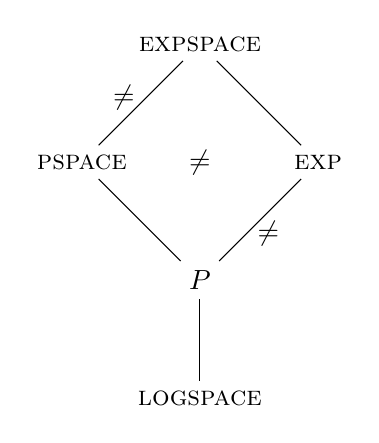
\begin{tikzpicture}
        \node (expspace) at (0,0) {$\textsc{expspace}$};
        \node (pspace) at (-1.5,-1.5) {$\textsc{pspace}$};
        \node (exp) at (1.5,-1.5) {$\textsc{exp}$};
        \node (p) at (0,-3) {$\mathbb{P}$};
        \node (logspace) at (0,-4.5) {$\textsc{logspace}$};
        \draw (expspace) -- (pspace) node [pos=0.7,above] {$\not=$};
        \draw (expspace) -- (exp);
        \draw (pspace) -- (p);
        \draw (exp) -- (p) node [pos=0.4,below] {$\not=$};
        \node () at (0,-1.5) {$\not=$};
        \draw (p) -- (logspace);
    \end{tikzpicture}
\end{document}
